\section{Analyses}
\label{sec:ablations}

To assess the robustness and practical implications of \method, we conduct a series of ablation studies that examine the impact of core methodological choices. These analyses investigate the following: \changed{(i) effectiveness of linear similarity measure, like cosine similarity, in capturing decoupling},  (ii) impact of the number of selected tokens, (iii) dependence on the choice of transformer layer, (iv) the influence of kernel type and kernel hyperparameters, (v) the effect of biased versus our adapted HSIC estimators, and (vi) the relative merits of different token selection strategies. The results, summarized below, reinforce the robustness of \method~across different design choices.

\subsection{Non-linear Dependence vs. Linear Similarity}\label{sec:hsic_vs_cos}
\changed{Table~\ref{tab:hsic_vs_cosine} compares HSIC with cosine similarity using both ranking-based (AUC$_s$) and correlation-based (PCC$_s$) metrics. On SQuAD, cosine similarity performs near random guessing, achieving low AUC$_s$ and negligible correlation with ground-truth labels, whereas HSIC attains substantially higher values on both metrics across models. On Natural Questions, cosine similarity exhibits highly variable behavior across models --- including strong AUC$_s$ in isolated cases but weak correlation --- while HSIC provides more stable performance across metrics. These results indicate that faithful input-output representations are not reliably aligned in a linear geometric sense, and that capturing non-linear statistical dependence is crucial for robust hallucination detection.
}

\begin{table}[t]
\small
\changed{
\centering
\begin{tabular}{llcccc}
\hline
& & \multicolumn{2}{c}{\textbf{SQuAD}} & \multicolumn{2}{c}{\textbf{NQ}} \\
\cline{3-6}
Model & Method & AUC$_s$ & PCC$_s$ & AUC$_s$ & PCC$_s$ \\
\hline
\multirow{2}{*}{Llama-3-8B}
& HSIC (\method) & \textbf{76.87} & \textbf{49.09} & \textbf{79.02} & \textbf{49.61} \\
& Cosine Similarity & 49.78 & 8.78 & 65.54 & 25.43 \\
\hline
\multirow{2}{*}{Gemma-2-9B}
& HSIC (\method) & \textbf{75.17} & \textbf{47.63} & 79.08 & \textbf{24.08} \\
& Cosine Similarity & 54.87 & 14.67 & \textbf{88.44} & 17.85 \\
\hline
\end{tabular}
\caption{\changed{Comparison of HSIC with cosine similarity for measuring input-output representational dependence on SQuAD and Natural Questions (NQ). HSIC consistently yields stronger ranking performance (AUC$_s$) and higher score-label correlation (PCC$_s$) on SQuAD, while cosine similarity exhibits unstable behavior across datasets and models.}}
\label{tab:hsic_vs_cosine}
}
\end{table}

\subsection{Impact of the Number of Selected Tokens}
\label{sec:token_budget}

% \begin{figure}[t!]
%     \centering
%     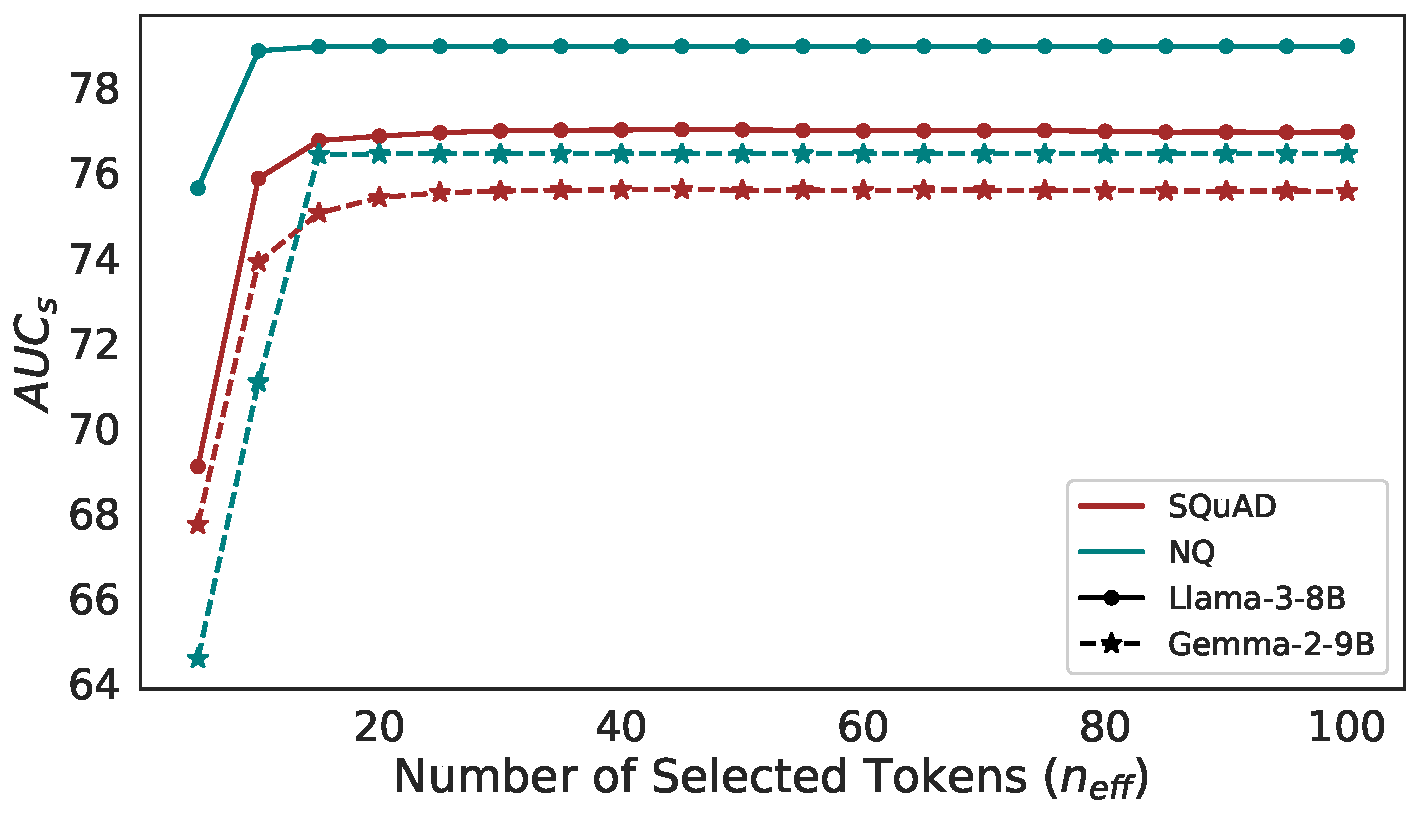
\includegraphics[width=0.6\columnwidth]{files/ablations/Keywords.pdf}
%     \caption{Variation in $AUC_s$ scores with the number of selected tokens used for \method-score calculation on the SQuAD and NQ datasets using Llama-3-8B and Gemma-2-9B. We observe that a token budget of $15-20$ results in a near-optimal performance, with diminishing gains upon further increase in $n_{\text{eff}}$.}
%     \label{fig:keyword_sensitivity}
% \end{figure}

\begin{figure}[t!]
    \centering
    \begin{minipage}{0.65\linewidth}  % Adjust width of figure
        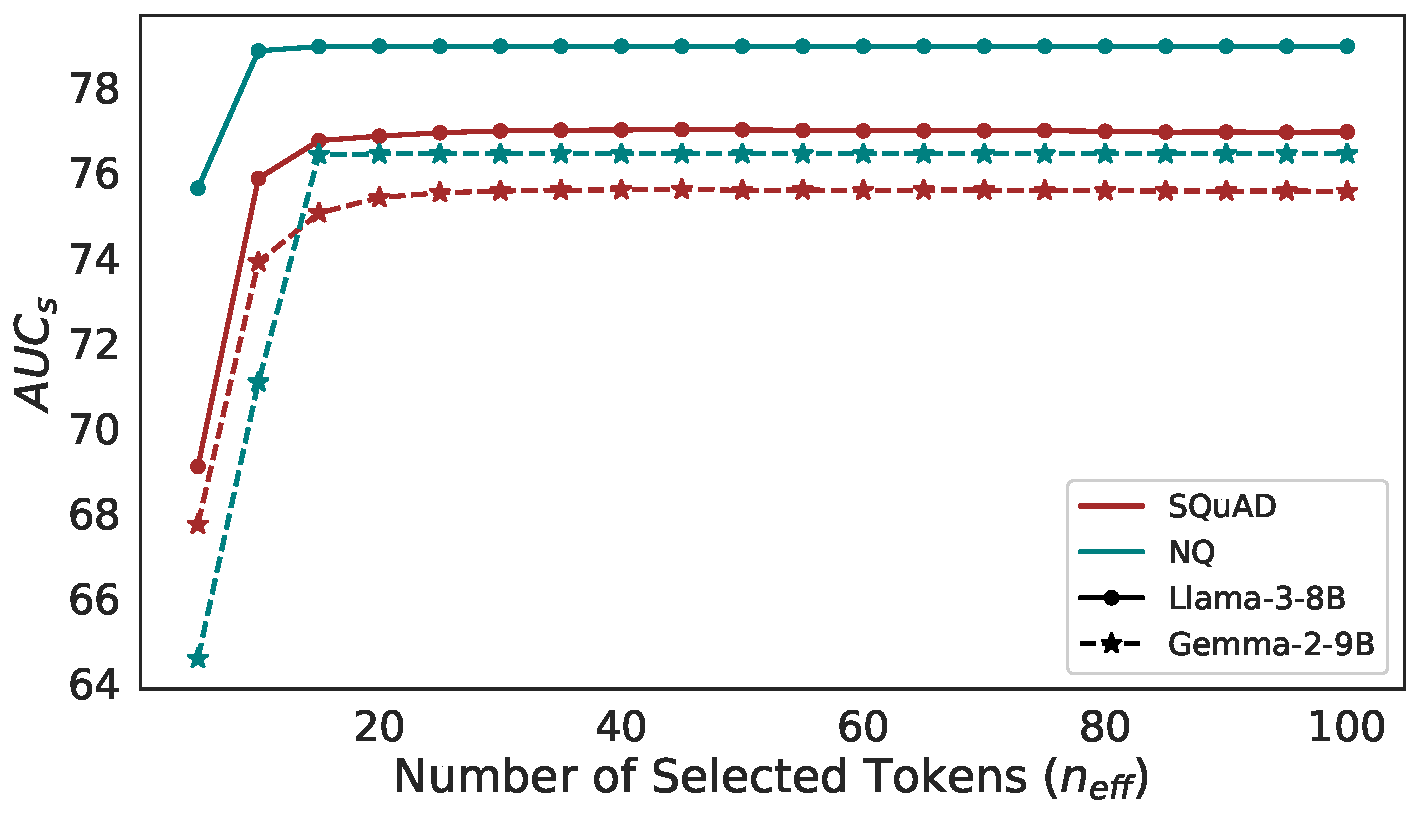
\includegraphics[width=\linewidth]{files/ablations/Keywords.pdf}
    \end{minipage}%
    \quad
    \begin{minipage}{0.3\linewidth}  % Adjust width of caption
        \caption{
        %Variation in $AUC_s$ scores with the number of selected tokens used for \method-score calculation on SQuAD and NQ datasets using Llama-3-8B and Gemma-2-9B. We observe that a token budget of $15$-$20$ results in a near-optimal performance, with diminishing gains upon further increase in $n_{\text{eff}}$.
        \changedtwo{Sensitivity analysis of detection performance to the token budget ($n_{eff}$). The detection performance ($AUC_s$) for both model families saturates at approximately $20$ tokens, suggesting that representational decoupling is a structural property that can be reliably estimated from a small subset of salient semantic pivots rather than requiring the full sequence length.}}
        \label{fig:keyword_sensitivity}
    \end{minipage}
\end{figure}


We begin by analyzing how the number of selected tokens ($n_{\text{eff}}$) affects detection performance. Figure~\ref{fig:keyword_sensitivity} illustrates that as $n_{\text{eff}}$ increases from $5$ to $10$, there is a clear improvement in the $AUC_s$ scores, but further increases beyond $15-20$ tokens result in diminishing returns. This levelling-off happened earlier for NQ across both models, likely because its shorter outputs often meant the actual number of tokens used was limited, regardless of a higher token budget. This finding holds consistently across datasets (SQuAD and NQ) and models (Llama-3-8B and Gemma-2-9B), indicating that \method~achieves near-optimal performance with a modest sample size. This property is practically significant, as it enables computational efficiency without sacrificing detection quality, even for outputs of varying lengths.


\subsection{Robustness to Selected Layer}\label{sec:layer_choice}

% \begin{figure}[t!]
%     \centering
%     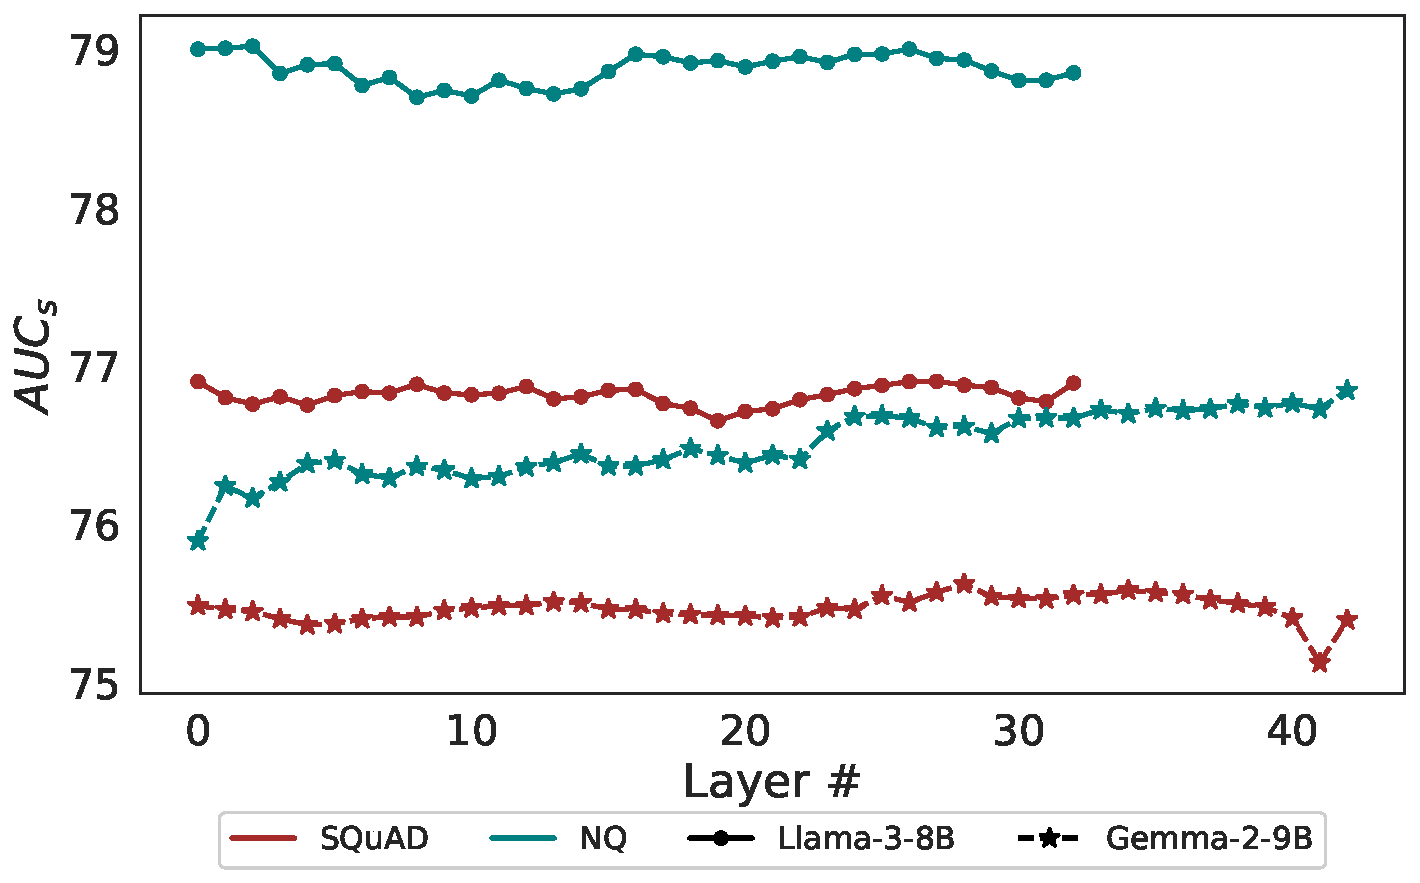
\includegraphics[width=0.6\columnwidth]{files/ablations/Layer.pdf}
%     \caption{Comparison of $AUC_s$ scores across different layers of LLama3-8B and Gemma-2-9B for both SQuAD and NQ datasets. We observe that the performance of \method~is almost agnostic to the chosen layer across models.}
%     \label{fig:layer_sensitivity}
% \end{figure}

Transformer architectures encode information at various abstraction levels across layers. To determine whether hallucination detection depends on the specific choice of decoder layer $\ell$, we systematically evaluate all 32 layers for Llama-3-8B and all 42 layers for Gemma-2-9B. As shown in Figure~\ref{fig:layer_sensitivity}, $AUC_s$ scores are stable across the full range of layers, with only minor fluctuations and a mild optimum near the network midpoint. Interestingly, neither model nor dataset exhibits significant performance drops at early or late layers that might be expected if hallucination detection using \method~required either low-level or high-level semantic features exclusively. This cross-architecture consistency suggests that the representational dependence signals captured by \method~are distributed throughout transformer networks rather than being concentrated in specific architectural regions, regardless of the underlying model design. 

\begin{figure}[t!]
    \centering
    \begin{minipage}{0.65\linewidth}  % Adjust width of figure
        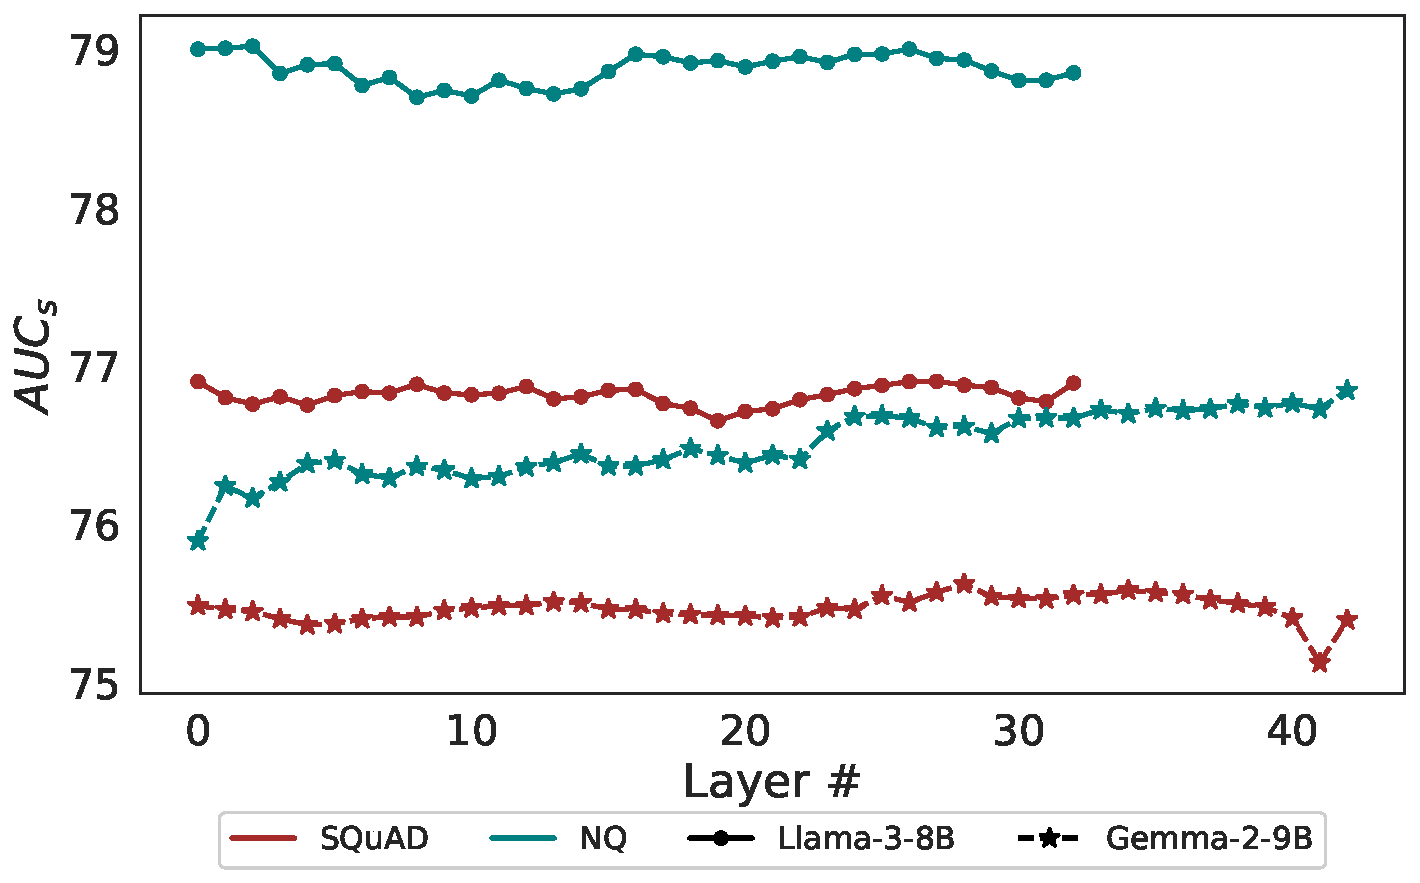
\includegraphics[width=\linewidth]{files/ablations/Layer.pdf}
    \end{minipage}%
    \quad
    \begin{minipage}{0.3\linewidth}  % Adjust width of caption
        \caption{%Comparison of $AUC_s$ scores when using representation from different layers of Llama-3-8B and Gemma-2-9B for \method-score calculation. We observe that the performance of \method~is almost agnostic to the chosen layer in case of both models, for both SQuAD and NQ datasets.
        \changedtwo{Consistency of the \method~signal across the full layer stack of Llama-3-8B and Gemma-2-9B. The stable $AUC_s$ scores across all layers indicate that representational decoupling is a globally distributed property of the transformer rather than an artifact localized to a specific architectural region, ensuring robust detection regardless of the target layer.}}
    \label{fig:layer_sensitivity}
    \end{minipage}
\end{figure}

\subsection{Effect of Kernel Function and RBF Hyperparameter}

\begin{figure}[t!]
    \centering
    \begin{subfigure}[b]{0.58\linewidth}
        \centering
        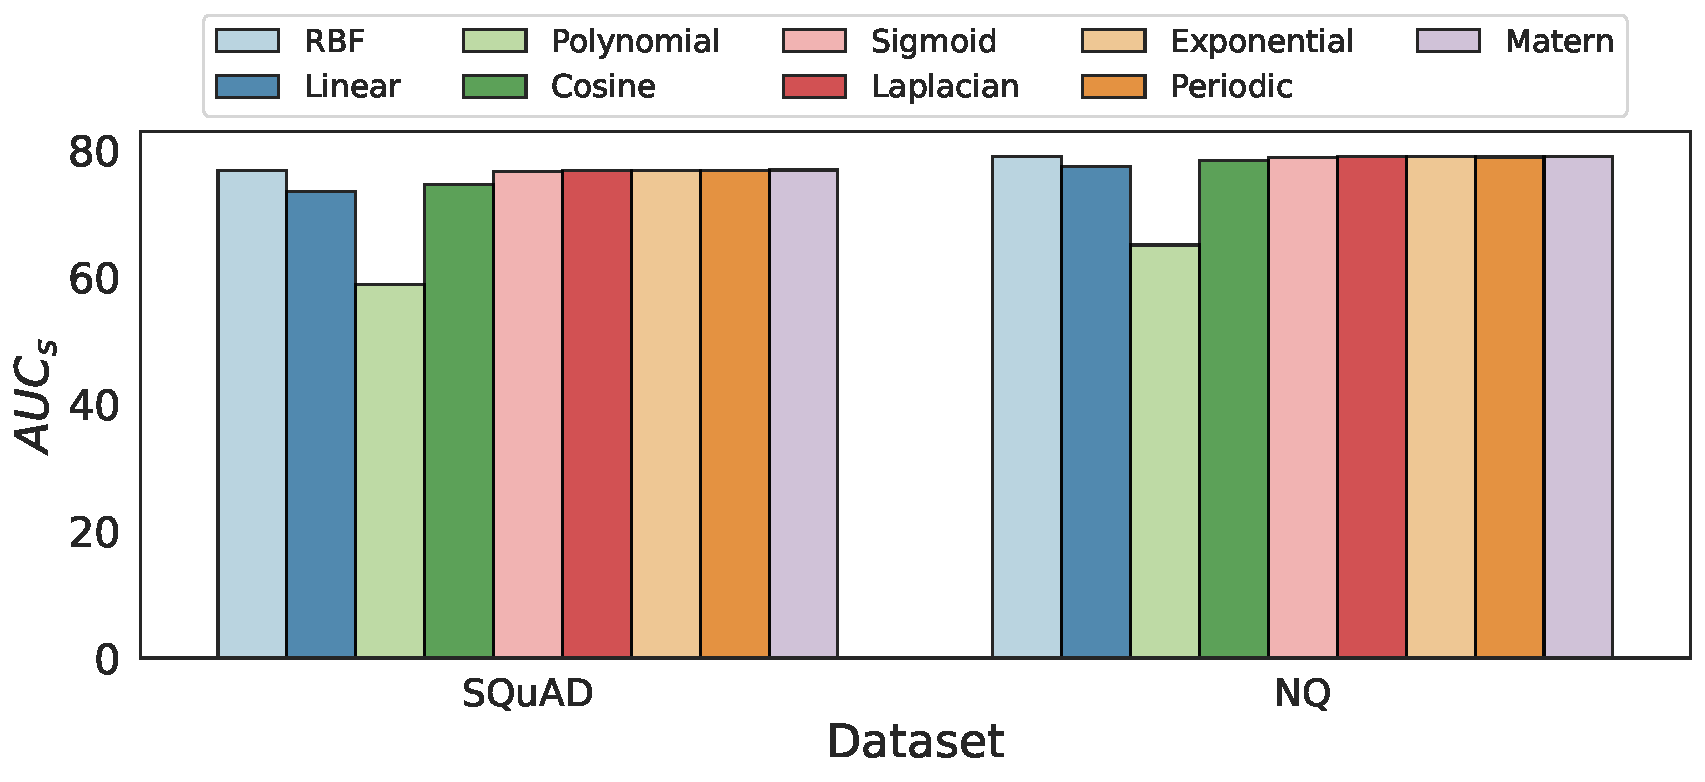
\includegraphics[width=\columnwidth]{files/ablations/Llama3-8B_kernel.pdf}
        \caption{}
        \label{fig:kernel_sensitivity}
    \end{subfigure}
    \begin{subfigure}[b]{0.41\linewidth}
    \centering
        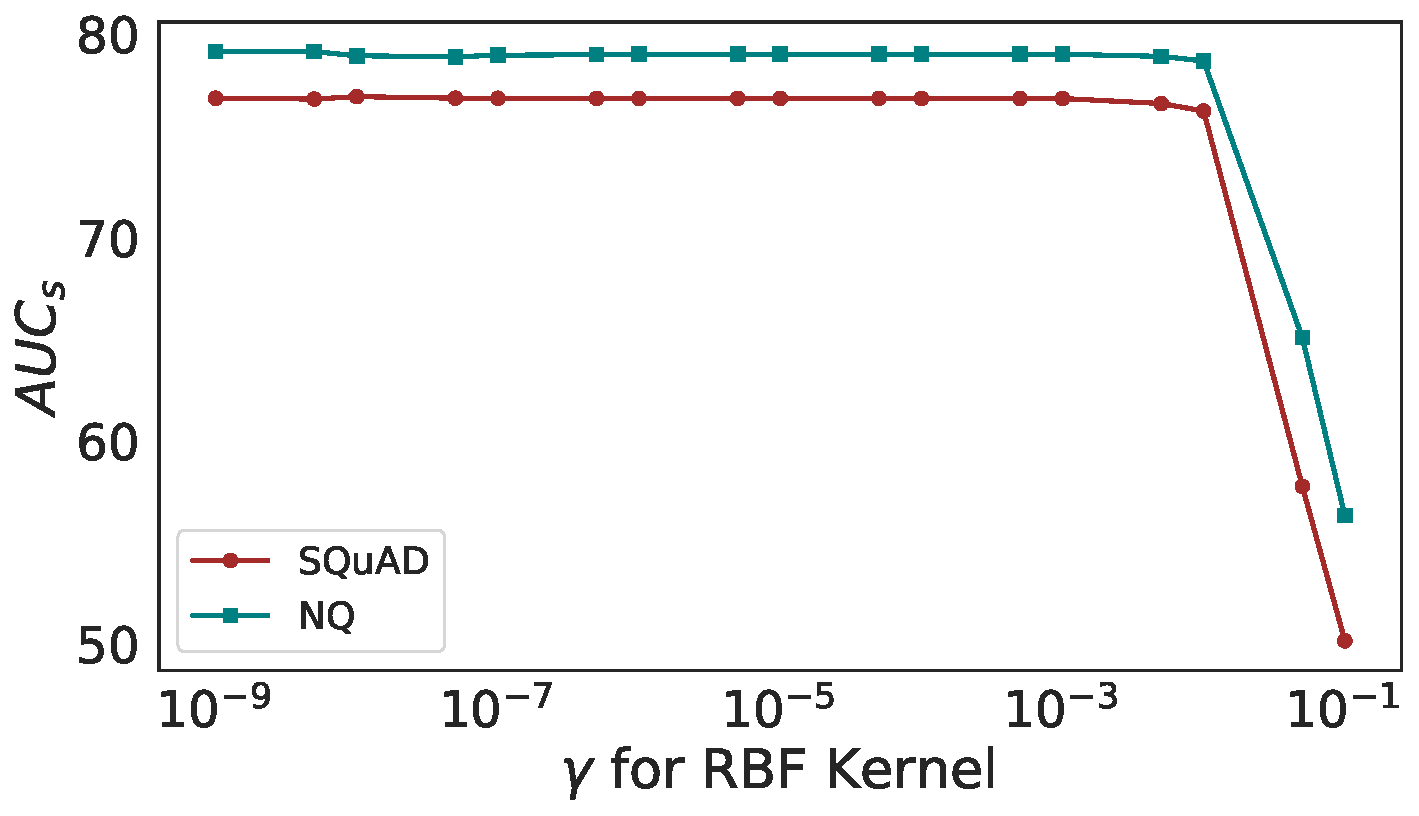
\includegraphics[width=\columnwidth]{files/ablations/Llama3-8B_Gamma.pdf}
        \caption{}
        \label{fig:gamma_sensitivity}
    \end{subfigure}
    \caption{Comparison of $AUC_s$ scores across (a) different kernel functions, and (b) different values of the hyperparameter $\gamma$ for the RBF kernel used for \method-score calculation on the SQuAD and NQ datasets using Llama-3-8B.}
    % \label{fig:kernel_sensitivity}
\end{figure}

Since \method~quantifies statistical dependence using HSIC, the choice of kernel function and its parameters is a critical consideration. We evaluate several kernel types -- including RBF (default), linear, polynomial, cosine, sigmoid, laplacian, exponential, periodic, and matern -- as well as a range of $\gamma$ values for the RBF kernel. 

Figure~\ref{fig:kernel_sensitivity} demonstrates that, with the exception of the polynomial kernel (which underperforms substantially), most kernels yield robust and similar $AUC_s$ scores for SQuAD and NQ, using Llama-3-8B. This suggests that the effectiveness of \method~is largely preserved regardless of kernel choice, with all kernels, except polynomial, providing strong performance.

For the RBF kernel, Figure~\ref{fig:gamma_sensitivity} shows that \method’s performance is stable across several orders of magnitude for $\gamma$ ($10^{-9}$ to $10^{-3}$), but degrades rapidly for larger values ($\gamma \geq 10^{-1}$). Excessively high $\gamma$ makes the kernel overly sensitive to minute differences in the hidden states, leading to overfitting and poor generalization. Conversely, smaller $\gamma$ values maintain a broader sensitivity that is more robust to natural variation in hidden representations. Together, these findings confirm that \method~is flexible to kernel choices and hyperparameters, but for optimal and consistent results, the RBF kernel with a moderate $\gamma$ remains a sound default.

\subsection{Effectiveness of HSIC Estimators}

\begin{figure}[t!]
    \centering
    \begin{minipage}{0.65\linewidth}  % Adjust width of figure
        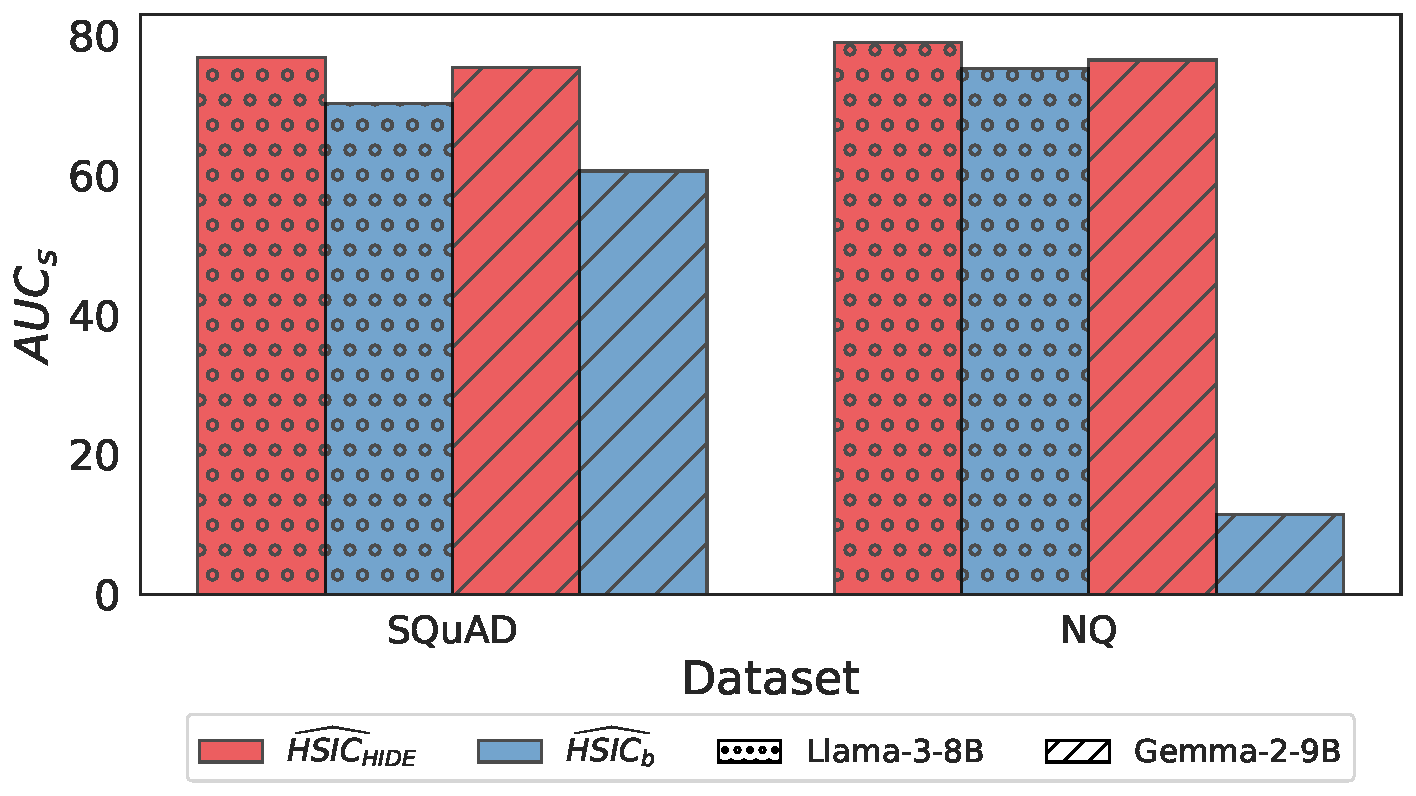
\includegraphics[width=\linewidth]{files/ablations/unbiased_biased.pdf}
    \end{minipage}%
    \quad
    \begin{minipage}{0.3\linewidth}  % Adjust width of caption
        \caption{%Comparison of $AUC_s$ scores using the biased estimator $\widehat{\operatorname{HSIC}}_b$ and our adapted estimator $\widehat{\operatorname{HSIC}}_{\method}$ for \method~score computation, for SQuAD and NQ datasets using LLama-3-8B and Gemma-2-9B.
        \changedtwo{Performance advantage of our adapted estimator ($\widehat{\operatorname{HSIC}}_{\method}$) over the biased baseline ($\widehat{\operatorname{HSIC}}_b$). The adapted estimator yields considerably higher $AUC_s$ scores by improving the separability between hallucinated and faithful generations, whereas the biased estimator compresses scores close to zero, making threshold determination unreliable.}}
    \label{fig:unbiased_biased}
    \end{minipage}
\end{figure}

% \begin{figure}[t!]
%     \centering
%     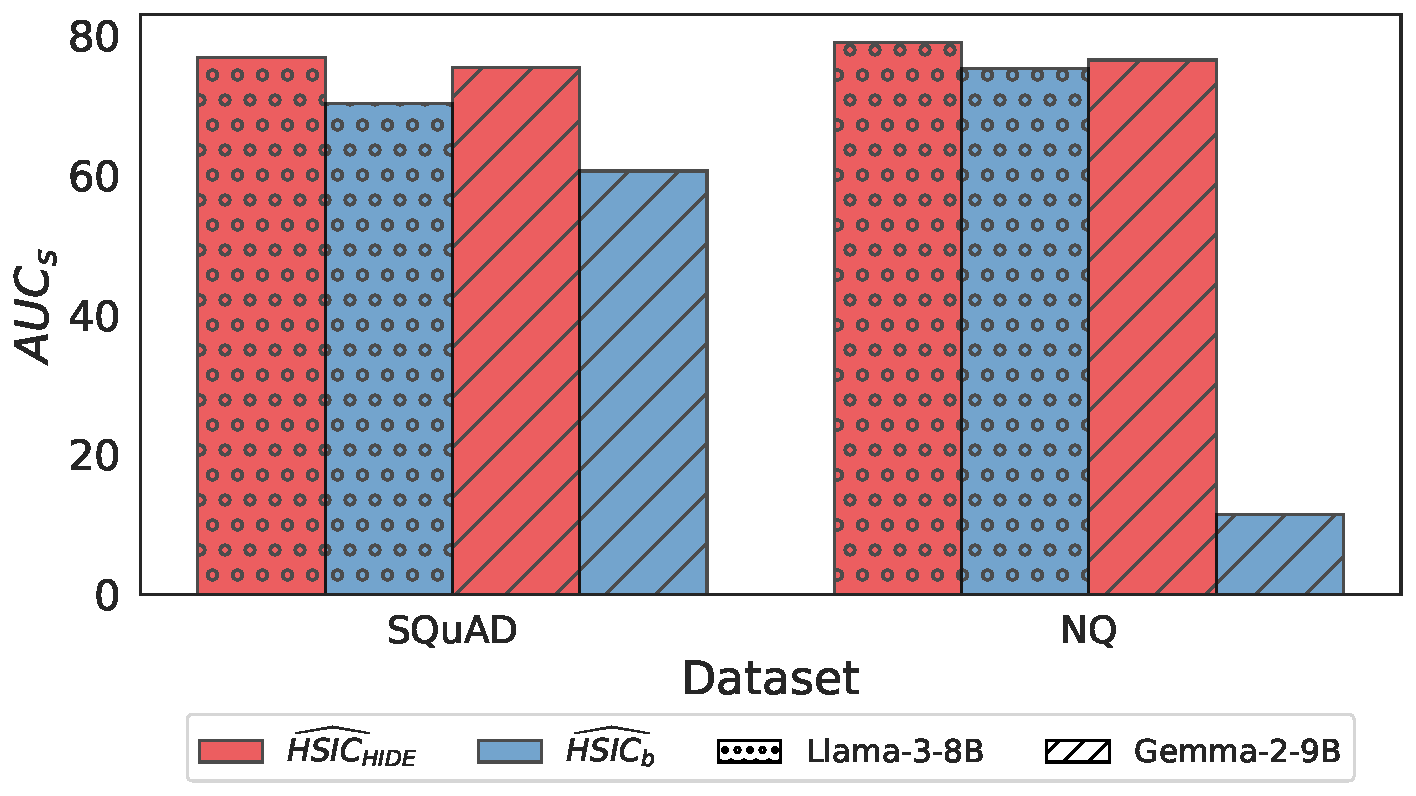
\includegraphics[width=0.6\columnwidth]{files/ablations/unbiased_biased.pdf}
%     \caption{Comparison of $AUC_s$ scores using the biased estimator $\widehat{\operatorname{HSIC}}_b$ and our adapted estimator $\widehat{\operatorname{HSIC}}_{\method}$ for \method~score computation, for SQuAD and NQ datasets using LLama-3-8B and Gemma-2-9B.}
%     \label{fig:unbiased_biased}
% \end{figure}

\begin{figure*}[t!]
    \centering
    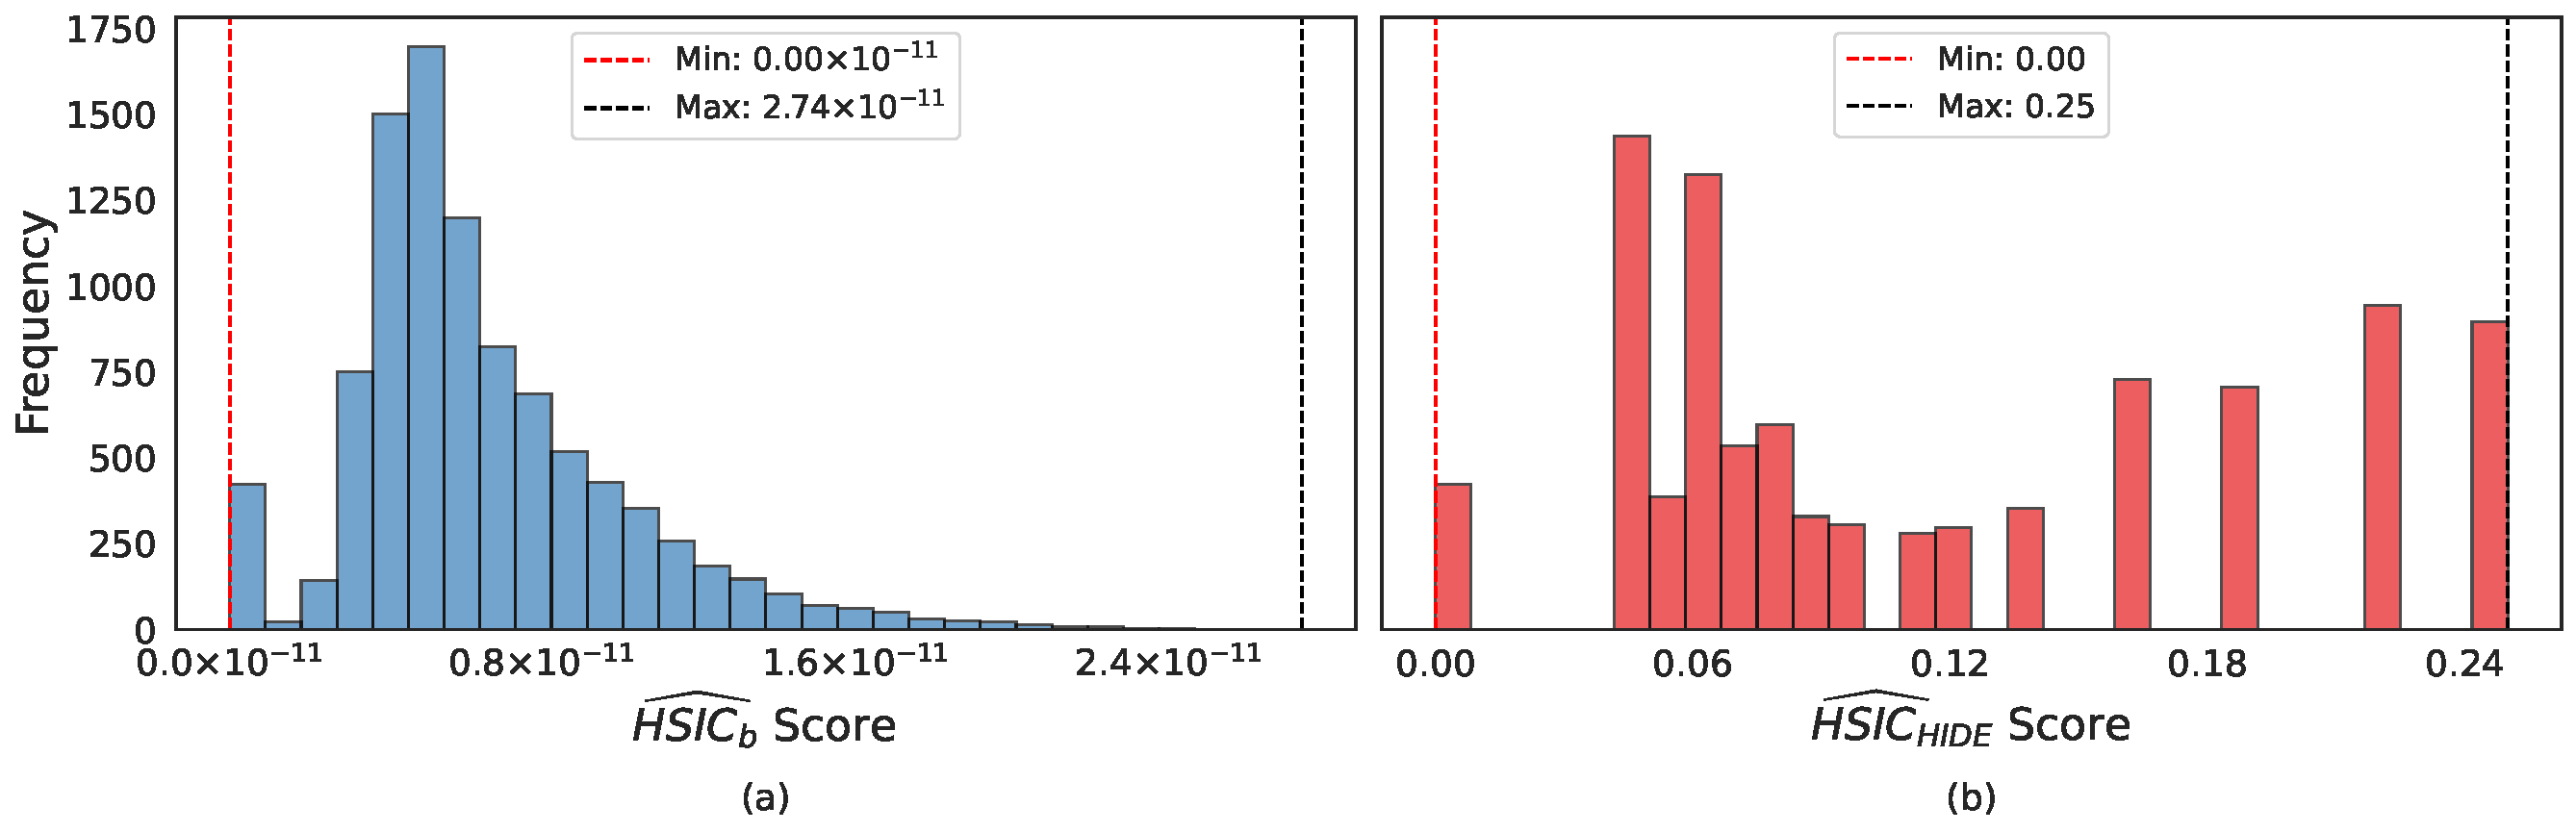
\includegraphics[width=\linewidth]{files/ablations/hsic_score_distributions.pdf}
    \caption{Distribution of \method~scores using $\widehat{\operatorname{HSIC}}_b$ and $\widehat{\operatorname{HSIC}}_{\method}$ estimators for HSIC calculation, for Llama-3-8B on SQuAD and NQ datasets.}
    \label{fig:score_distribution}
\end{figure*}
We compare the performance of \method~with the biased estimator, $\widehat{\operatorname{HSIC}}_b$, and our adapted estimator $\widehat{\operatorname{HSIC}}_{\method}$, for empirical HSIC computation, as shown in Figure~\ref{fig:unbiased_biased}. $\widehat{\operatorname{HSIC}}_{\method}$ delivers consistently higher performance across datasets and models, owing to improved score separability between hallucinated and faithful generations. As shown in Figure \ref{fig:score_distribution}, $\widehat{\operatorname{HSIC}}_{\method}$ produces a more favourable score distribution spanning $0-0.25$, creating clearer separation between hallucinated and non-hallucinated generations. In contrast, $\widehat{\operatorname{HSIC}}_b$ yields extremely small values, compressing scores close to zero (with a maximum score of $2.74\times10^{-11}$), making threshold determination challenging and less reliable. Therefore, we adopt $\widehat{\operatorname{HSIC}}_{\method}$ for our framework.


\subsection{Impact of Token Selection Strategies}
\label{sec:token_selection}
Finally, we compared two strategies for selecting token representations (as discussed in \cref{sec:token_alignment}): keyword-based selection and SVD-based alignment. Figure~\ref{fig:svd_keyword} shows that both approaches perform nearly identically across datasets and architectures. The SVD method guarantees mathematical orthogonality, while the keyword-based approach enhances interpretability by enabling semantic traceability -- allowing users to attribute detection decisions to specific content elements. Given this enhanced transparency of the keyword-based strategy and the absence of any performance penalty, we adopt the keyword-based selection as the default for \method.

\begin{figure}[t!]
    \centering
    \begin{minipage}{0.65\linewidth}  % Adjust width of figure
        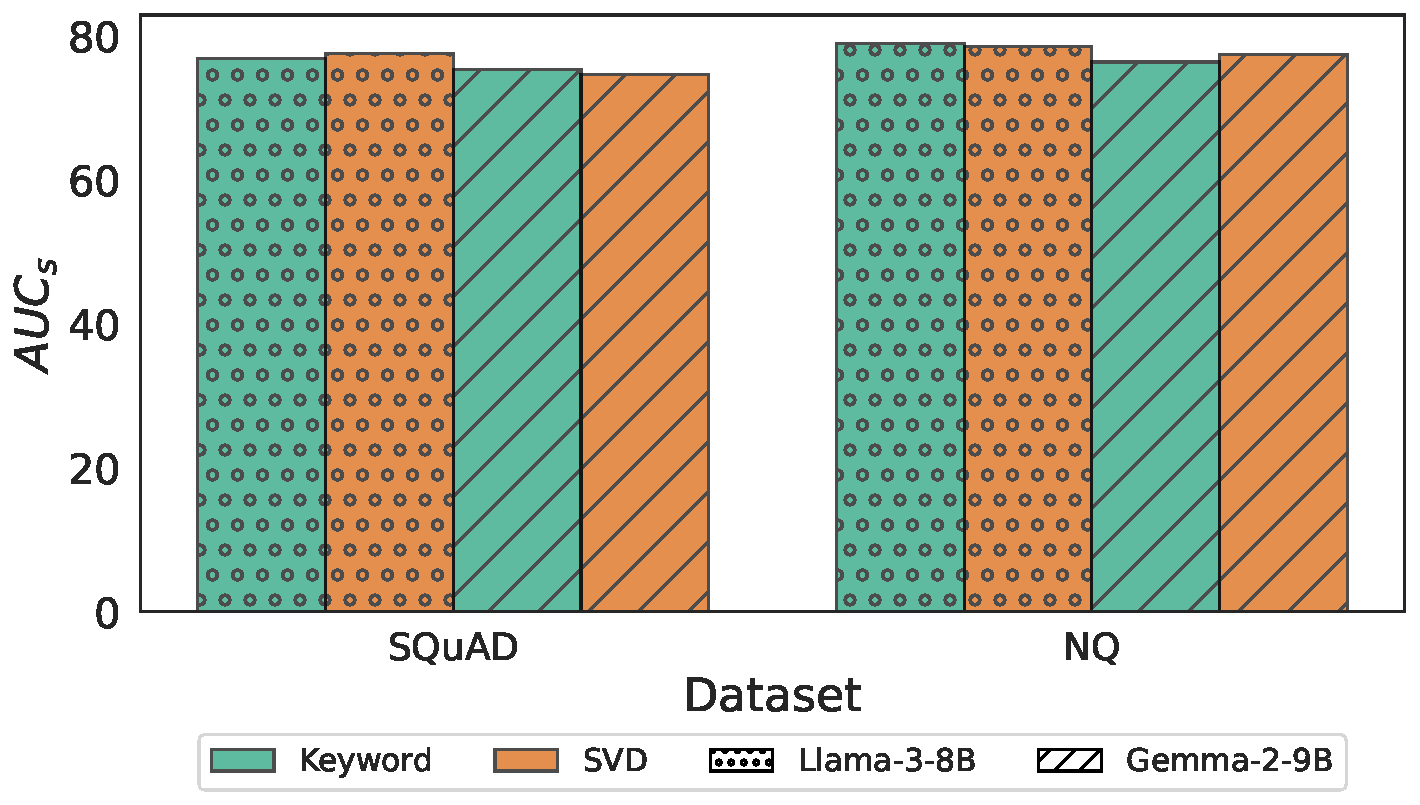
\includegraphics[width=\linewidth]{files/ablations/svd_keyword.pdf}
    \end{minipage}%
    \quad
    \begin{minipage}{0.3\linewidth}  % Adjust width of caption
        \caption{Comparison of $AUC_s$ scores for keyword-based and SVD-based token selection strategies, for SQuAD and NQ datasets using Llama-3-8B and Gemma-2-9B.}
    \label{fig:svd_keyword}
    \end{minipage}
\end{figure}

% \begin{figure}[t!]
%     \centering
%     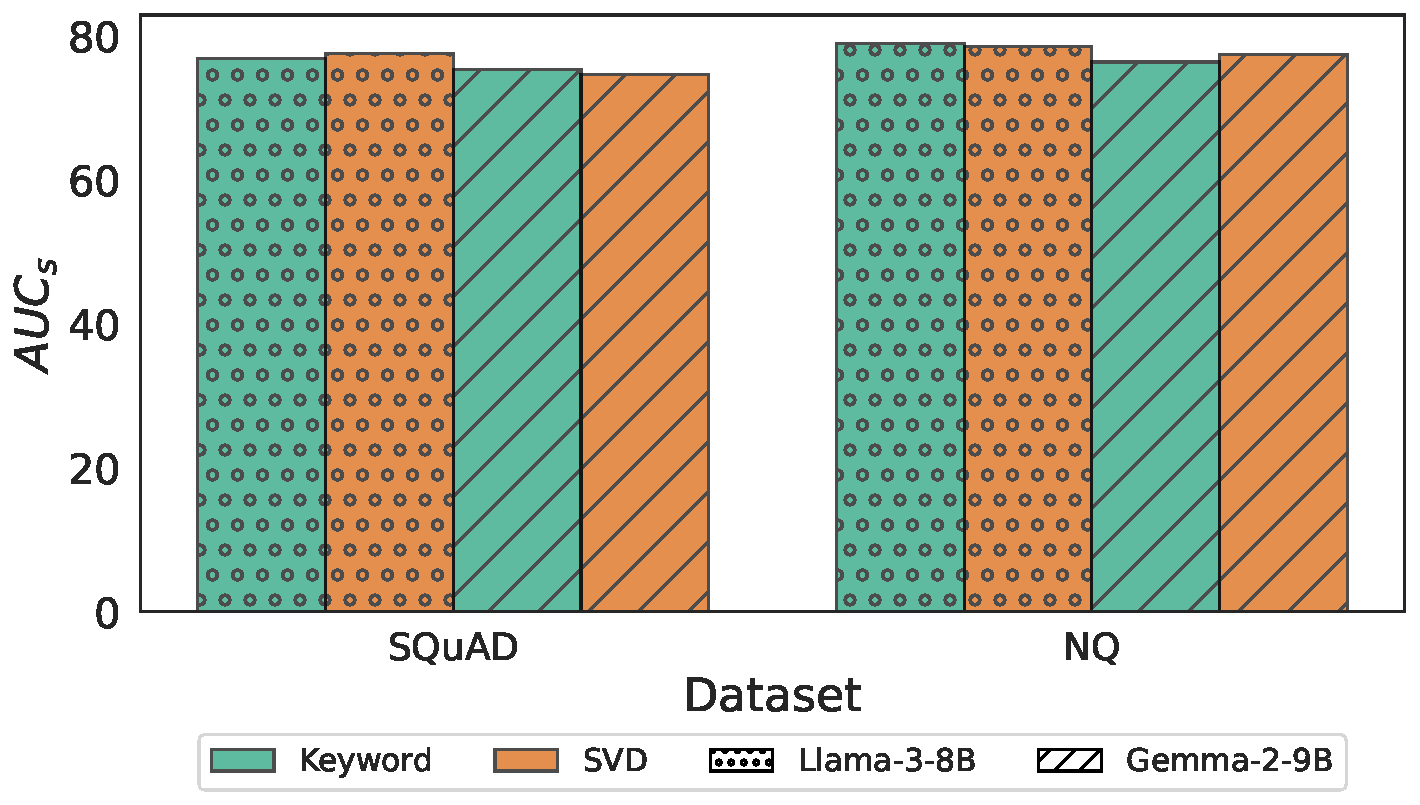
\includegraphics[width=0.6\columnwidth]{files/ablations/svd_keyword.pdf}
%     \caption{Comparison of $AUC_s$ scores for keyword-based and SVD-based token selection strategies, for SQuAD and NQ datasets using LLama-3-8B and Gemma-2-9B.}
%     \label{fig:svd_keyword}
% \end{figure}

\subsection{Qualitative Analysis of Representational Decoupling}
\begin{table}[t]
\centering
\small
\begin{tabular}{p{2cm} p{1.8cm} p{1.5cm} p{1.2cm} p{1.2cm} c c}
\hline
\textbf{Prompt (Dataset)} &
\textbf{Input Keywords} &
\textbf{Output Keywords} &
\textbf{Model Output} &
\textbf{Gold Answer} &
\textbf{\method~Score} &
\textbf{Hallucinated?} \\
\hline
Who had a 70s No.1 hit with \emph{Kiss You All Over}? \textbf{(TriviaQA)} &
\emph{70s hit, Kiss You All Over, song} &
\emph{Exile, band, hit} &
Exile &
Exile &
0.182 &
No \\\hline

What claimed the life of singer Kathleen Ferrier? \textbf{(TriviaQA)} &
\emph{Kathleen Ferrier, singer, death} &
\emph{cancer, illness} &
Cancer &
Cancer &
0.164 &
No \\\hline

Who was the man behind The Chipmunks? \textbf{(TriviaQA)} &
\emph{The, Chipmunks, Who, ...} &
\emph{Bagdasarian, Songbook, Ross, name, first, Sr, ...} &
Ross Bagdasarian, Sr. &
David Seville &
0.066 &
Yes \\\hline

What is the capital of Australia? \textbf{(NQ)} &
\emph{Australia, capital} &
\emph{Sydney, city} &
Sydney &
Canberra &
0.034 &
Yes \\
\hline
\end{tabular}
\caption{
\changed{Qualitative examples illustrating representational coupling and decoupling for Llama-3-8B.
Faithful generations exhibit strong alignment between salient input and output concepts,
resulting in high \method~scores. Hallucinated generations introduce unsupported entities or
semantic drift, leading to substantially lower dependence scores.
}}
\label{tab:qualitative_examples}
\end{table}

\changed{
Table~\ref{tab:qualitative_examples} illustrates how representational decoupling aligns with
hallucination behavior. Faithful generations preserve alignment between salient input and
output concepts, yielding high HIDE scores. Hallucinated outputs introduce unsupported
entities or semantic drift, resulting in substantially lower dependence scores. This
contrast provides qualitative intuition for why HSIC-based dependence captures hallucinations
beyond surface-level similarity. Several more illustrative examples from different datasets are presented in Appendix D.
}


\subsection{Robustness to Decoding Strategies}
\label{sec:decoding_strategies}
\changedtwo{
Autoregressive internal dynamics and hallucination rates are known to vary across different decoding regimes. Theoretically, HIDE's effectiveness is decoupled from the specific token-selection mechanism. If a stochastic sampling choice forces the generation off-topic or into a parametric hallucination, the output representations structurally diverge from the input context, and the HSIC score should reliably reflect this decoupling. 
}

\changedtwo{
To empirically validate this, we evaluated HIDE across multiple temperature ($T \in \{0.3, 0.6, 0.9\}$) and nucleus sampling ($Top\text{-}p \in \{0.7, 0.8, 0.9\}$) configurations on SQuAD and Natural Questions. As detailed in Table \ref{tab:decoding_robustness}, HIDE exhibits remarkable stability across all settings. The $AUC_s$ and $PCC_s$ scores remain consistently strong, and in several stochastic configurations, performance marginally improves over the greedy baseline. This confirms that representational decoupling is a robust, generation-agnostic signal.
}

\begin{table}[h]
\centering
\small
\resizebox{\columnwidth}{!}{%
\begin{tabular}{llcccc}
\toprule
\multirow{2}{*}{\textbf{Model}} & \multirow{2}{*}{\textbf{Decoding Strategy}} & \multicolumn{2}{c}{\textbf{SQuAD (Faithfulness)}} & \multicolumn{2}{c}{\textbf{NQ (Factuality)}} \\ \cmidrule(lr){3-4} \cmidrule(lr){5-6}
 & & \textbf{AUC$_s$} & \textbf{PCC$_s$} & \textbf{AUC$_s$} & \textbf{PCC$_s$} \\ \midrule
\multirow{7}{*}{Llama-3-8B} 
 & Greedy & 76.87 & 49.09 & 79.02 & 49.61 \\
 & $T=0.3$ & 77.02 & 49.61 & 79.32 & 49.93 \\
 & $T=0.6$ & 79.58 & 52.44 & 77.90 & 45.64 \\
 & $T=0.9$ & 80.74 & 53.02 & 81.37 & 48.40 \\
 & $Top\text{-}p=0.9$ & 79.63 & 51.17 & 78.12 & 44.68 \\
 & $Top\text{-}p=0.8$ & 79.09 & 50.70 & 81.82 & 46.85 \\
 & $Top\text{-}p=0.7$ & 79.62 & 52.35 & 80.13 & 47.79 \\ \midrule
\multirow{7}{*}{Gemma-2-9B} 
 & Greedy & 75.17 & 47.63 & 79.08 & 24.08 \\
 & $T=0.3$ & 75.72 & 47.48 & 80.97 & 34.85 \\
 & $T=0.6$ & 76.89 & 48.46 & 81.84 & 42.70 \\
 & $T=0.9$ & 76.41 & 46.20 & 78.28 & 44.21 \\
 & $Top\text{-}p=0.9$ & 77.95 & 47.22 & 75.88 & 42.76 \\
 & $Top\text{-}p=0.8$ & 78.09 & 47.41 & 77.84 & 42.86 \\
 & $Top\text{-}p=0.7$ & 77.15 & 47.79 & 76.41 & 44.04 \\ \bottomrule
\end{tabular}%
}
\caption{\changedtwo{Robustness of HIDE across various decoding regimes. Performance remains highly stable across greedy and stochastic generation strategies.}}
\label{tab:decoding_robustness}
\end{table}